\documentclass[../thesis]{subfiles}

\begin{document}
	\section{Results}
	\label{sec:mic:results}

	Performance tests focused mainly on the the optimizations described in \cref{subsec:mic:optims:blockified,subsec:mic:optims:self} (\emph{blockified} and \emph{self}). Premature tests revealed that the first optimization (massive parallelism) did not decrease the execution time of the algorithm, and the benefit from the second optimization (loop unrolling) was too little to be significant. Although this was not the case with the third optimization (removed Armadillo), since it required a major change to the implementation, it was used as the base for \emph{blockified} and \emph{self}. When reading the following results, it is important to consider that a significant fraction of the improvements shown by these optimizations comes from that.

	Theoretically, the parallelization of the dependency solving step compensates for the lack of parallelism in the more advanced stages of the algorithm. However, tests shown this not to be the case. Initially, the memory access pattern was blamed. As the algorithm progresses, the number of dependencies for each element increase, but half of this dependencies lie in distinct cache lines. The lack of locality was thought to be at fault, hampering so much the algorithm that it would nullify any improvement from increased parallelism.

	Subsequent research \cite{PRACE:MIC:BestPracticeGuide} revealed the problem to be in the way OpenMP was being used. It was assumed that threads would automatically be spread amongst nested parallel regions, similar to what happens with the scheduling of threads in a single parallel region, but the truth is that nested parallelism is disabled by default. Consequently, it has to be enabled manually, either through the environment or through a small change in the source code. Additionally, the number of threads for each parallel region also has to be set manually, either through the environment (using comma separated values) or by using the default OpenMP routine to set the number of threads for each region individually. Despite the correction being fairly easy, when the problem was correctly identified there was no time left to rerun the performance tests.

	On the other hand, the lack of performance improvements from the loop unrolling optimization did not come as a surprise, serving the purpose of proving how the \intel\xeonphi coprocessor is superior to a \gpu when dealing with conditionals.

	The execution time for the \emph{blockified} optimization is shown in \cref{fig:mic:optims:blockified:times}. Comparing with \cref{fig:mic:block:diagonal:times}, the sequential time was reduced to less than half. The peak performance kept near the same number of threads (30 for $n=2000$, 60 for $n=4000$ and 120 for $n=8000$). When more threads than those supported by the hardware are demanded, the performance now drops more intensely, with the optimized implementation taking twice as long with 360 threads.

	\begin{figure}[p]
		\begin{center}
			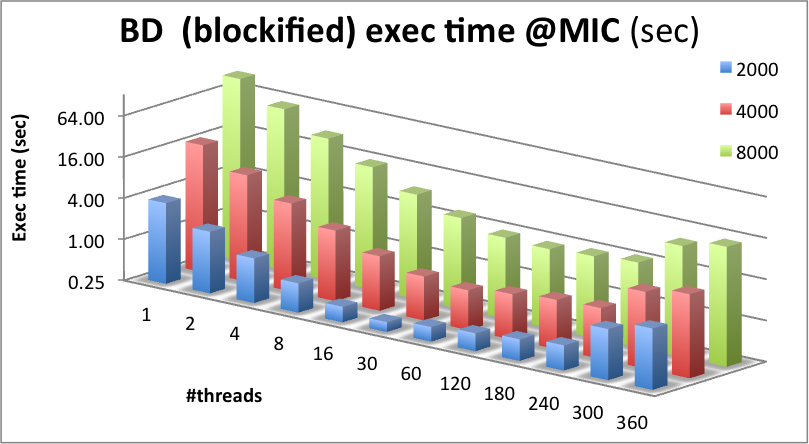
\includegraphics[width=0.9\textwidth]{assets/images/mic/optims/mic-blockified.png}
		\end{center}
		\caption{Execution times for the \emph{blockified} optimization in the \intel\xeonphi coprocessor.}
		\label{fig:mic:optims:blockified:times}
	\end{figure}

	While not so good, the \emph{self} optimization also improves the efficiency of the implementation, as shown in \cref{fig:mic:optims:self:times}. Contrary to what happens with \emph{blockified}, this optimization practically removes the penalty of demanding more threads than what the hardware supports, maintaining the execution time near peak performance even above 8 threads per core. Yet, the minimum execution time this optimization achieves is not as low.

	\begin{figure}[p]
		\begin{center}
			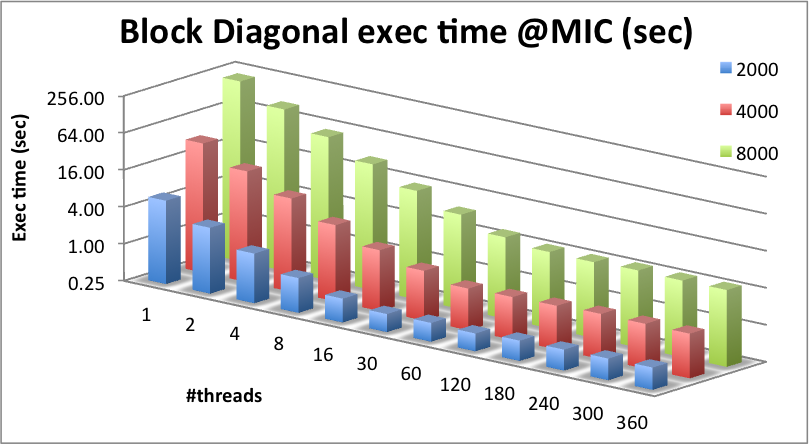
\includegraphics[width=0.9\textwidth]{assets/images/mic/optims/mic-self.png}
		\end{center}
		\caption{Execution times for the \emph{self} optimization in the \intel\xeonphi coprocessor.}
		\label{fig:mic:optims:self:times}
	\end{figure}

	Although \emph{blockified} exceeds \emph{self} in speedup, the highest efficient is achieved when using both optimizations at the same time (\cref{fig:mic:optims:blockified_self:times}). The sequential time and the time obtained with 360 threads are practically the same as for \emph{blockified} only, and the same happens for the peaks. However, the value obtained with these peaks is reduced when \emph{self} is also applied.

	\begin{figure}[p]
		\begin{center}
			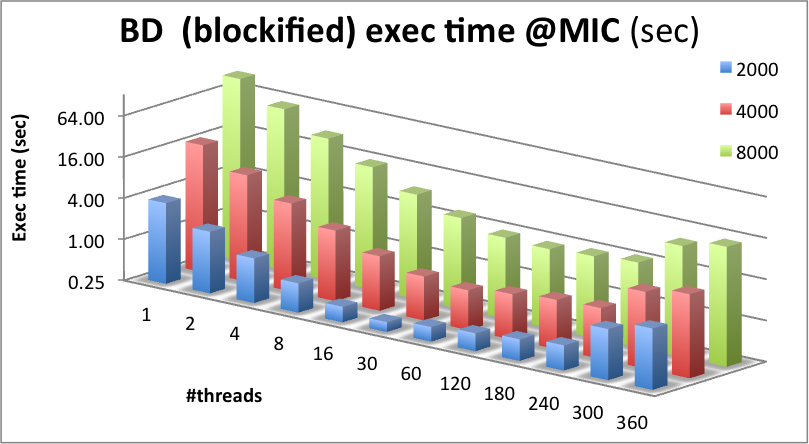
\includegraphics[width=0.9\textwidth]{assets/images/mic/optims/mic-blockified.png}
		\end{center}
		\caption{Execution times for \emph{blockified} and \emph{self} in the \intel\xeonphi coprocessor.}
		\label{fig:mic:optims:blockified_self:times}
	\end{figure}

	\Cref{fig:mic:optims:best:times} shows the best execution times for the naive implementation and each optimization running in the \intel\xeonphi and the best execution time for \emph{blockified} and \emph{self} together running on the multicore environment. While it is clear the benefit of both optimizations, there is the problem of these optimizations being common to both the coprocessor and the multicore environment. However, \cref{fig:mic:optims:best:times} shows that these optimizations reduce significantly the speedup gap between the \cpu and the device.

	\begin{figure}[p]
		\begin{center}
			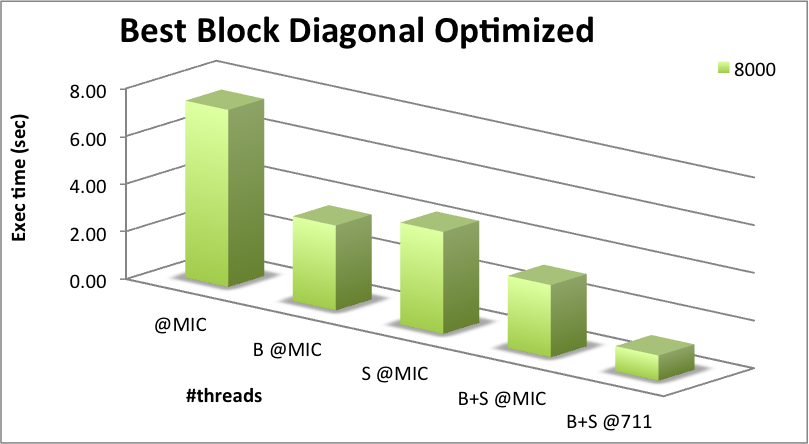
\includegraphics[width=0.9\textwidth]{assets/images/mic/optims/best.png}
		\end{center}
		\caption{Best execution times for the optimizations. \emph{B} means \emph{blockified}, \emph{S} means \emph{self}.}
		\label{fig:mic:optims:best:times}
	\end{figure}

	\begin{figure}[p]
		\begin{center}
			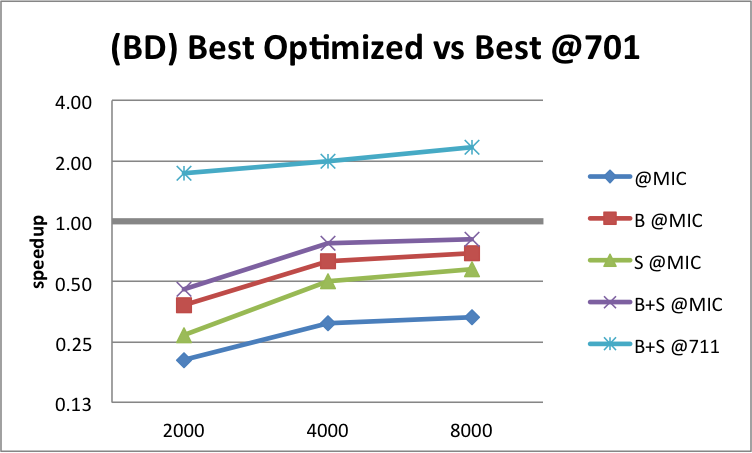
\includegraphics[width=0.9\textwidth]{assets/images/mic/optims/best-speedup.png}
		\end{center}
		\caption{Speedups for the optimizations versus multicore in group 701. \emph{B} means \emph{blockified}, \emph{S} means \emph{self}.}
		\label{fig:mic:optims:best:speedup}
	\end{figure}
\end{document}
